\documentclass[a4paper, 11pt, titlepage]{jsarticle}
\usepackage[dvipdfmx]{graphicx}
\usepackage{listings}
\usepackage{amsmath}
\usepackage{url}

\title{知能情報実験III(データマイニング班)\\顔判別システム}
\author{185716K,185718F,185728C,185741A}
\date{提出日:2020年8月12日}
\begin{document}
\maketitle
\tableofcontents
\clearpage

\section{はじめに}
\subsection{実験の目的と達成目標}
知能情報実験IIIは、情報工学分野のより専門的な知識を理解・習得することを目的として、半年間でシステムの開発やデータ解析等に取り組む実施される。
その中の一つデータマイニング班においては機械学習外観ならびにその応用を通し、対象問題への理解、特徴量抽出等の前処理、バージョン管理やデバッグ・テスト等を含む仕様が定まっていない状況下における開発方法、コード解説や実験再現のためのドキュメント作成等の習得を目指す。

\subsection{顔判別システムとは}
本グループでは自身が有名人の誰に似ているかを教師あり学習を用いて顔判別をすることを対象 問題として設定した。今実験では、目や鼻、口、輪郭の位置関係から顔を識別し、その差異によって顔判別を実施した。上記の顔のパーツを検出できる学習済みのファイルであるhaarcascadeを使って、嵐のメンバーと自分の顔写真の顔パーツを認識する。そのデータを用いて、自分が嵐のメンバーの誰に似ているかをこの開発の最終目標とした。

\section{実験方法}
\subsection{実験目的}
実際にOpenCV等のツールを用いつつ機械学習を行うことによって顔認証の精度を測定し、その向上の方法を考察する。また、この実験を通して機械学習への理解を深める。

\subsection{実験計画}
実際に実施した実験計画の順序を下記1$\sim$4に示す。
\begin{enumerate}
\item{嵐5人それぞれの画像を収集する。}
\item{嵐の各メンバーに対して顔全体の検出を行い、本人の顔データだけのデータセットを構築
する。}
\item{2のデータを学習させて顔識別を行い、嵐のメンバーがその通りに認識されるかを検証する。
(精度向上)}
\item{他人の顔写真がメンバーの誰に似ているかを正しく判断することができるかを検証する。}
\end{enumerate}

\subsubsection{なぜパーツごとに識別しようと考えたか}
顔全体と顔の各パーツごとに識別しようと考えた理由として、人の顔は各パーツごとに特徴を
持っているので、パーツごとに細分化することによってより最適な結果が得られると仮定した。

\subsection{データセット構築}
データセット構築の処理順序を下記$\sim$に示す。

\begin{enumerate}
\item{icrawlerで画像の収集。}
\item{OpenCVを利用して顔(瞳)部分を抽出し、抜き出す。}
\item{不要な画像、顔以外が抜き出された画像の削除。}
\item{画像処理での、画像の水増し。}
\end{enumerate}

\subsubsection{データの水増し方法}
Pythonを用いて、学習画像を1枚ずつそれぞれ垂直方向への反転、90度回転、270度回転、グレー化、ヒストグラムの変更した画像分を増量させた。

\subsection{モデル選定}
今回の実験では、VGG16を活用してfine tuningすることで機械学習を進めた。VGG16というのは,「ImageNet」と呼ばれる大規模画像データセットで学習された,16層からなるCNNモデルのことで、kerasにはVGG16の学習済みモデルが標準的に設定されているため、それを利用した。1000カテゴリに分類した畳み込みニューラルネットワークのモデルであるVGG16を活用してその学習済モデルを、重みデータを一部再学習して特徴量抽出機として利用するfine tuningを使って機械学習を実行した。その理由としては、他の画像データを使って学習されたモデル(VGG16)を使うことによって、新たに作るモデルは少ないデータ・学習量でモデルを生成することが可能となるためである。本実験では、あまり多くのデータ量を集めることができなかったため、fine tuningを利用することで、精度向上を試みた。

\subsection{パラメータ調整}
本実験で設定したパラメータ調整について説明する。各メンバーのサンプル総数は集められたデータが嵐5人の中で一番少ないメンバーに合わせて1000個に統合した。その中から、ホールドアウト法を用いて、データ全体を学習用データとテストデータに分割を行った。1000個のデータのうち8割の800個をトレーニング用データとして、2割をバリデーション用データとして使用した。この割合は少ない割合から実験開始したが、2割で学習がうまくいったため、この割合のまま進行した。バッチサイズは機械学習の分野の慣習1として2のn乗の値が使われるため、32、64と試したがほとんど変化はなく優れた数値を得ることができたので、本実験でのバッチサイズは32とした。画像サイズは参考サイトのコード通りの$150\times 150$にして問題ないと判断したためこのサイズのまま実験を進めた。

\subsection{学習結果}
エポック数を100に設定して嵐の顔データを学習させた結果は図\ref{fig1}のようになり、95\%以上とかなり良い精度が得られた。

\begin{figure}[htbp]
 \centering
  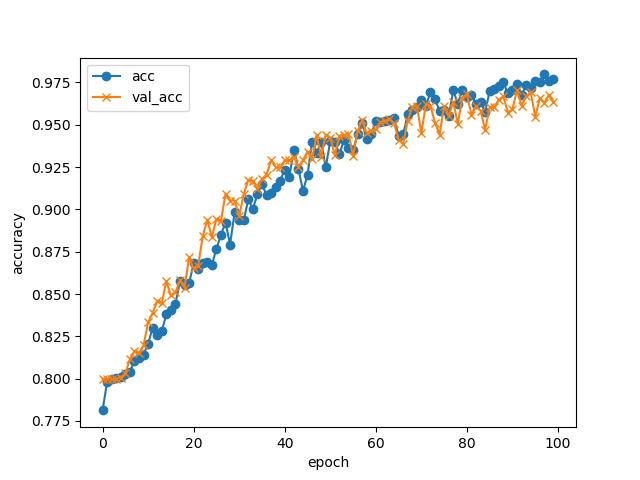
\includegraphics[width=120mm]{graph1}
  \caption{学習結果}
  \label{fig1}
\end{figure}

\section{実験結果}
\begin{enumerate}
\item{嵐本人の顔で認証を行なった場合}\\
本人の画像で認証した結果は下記のようになった。桜井翔以外は 98\%以上とかなり良い結果が出た。だが、櫻井翔だけは75\% と他メンバーと比較して低い結果となった。\\
\begin{itemize}
\item{相葉雅紀の画像}\\
'松本潤':0,'二宮和也':1,'相葉雅紀':2, '櫻井翔':3, '大野智':4
 
[0.01277803\ 0.00011003\ 99.97391\ 0.01296918\ 0.00023498]\ $\rightarrow$ 約99\%
\item{大野智の画像}\\
'松本潤':0,'二宮和也':1,'相葉雅紀':2, '櫻井翔':3, '大野智':4

[0.00022745\ 0.08343612\ 0.00024487\ 0.00024956\ 99.91584]\ $\rightarrow$ 約99\%
\item{櫻井翔の画像}\\
'松本潤':0,'二宮和也':1,'相葉雅紀':2, '櫻井翔':3, '大野智':4

[0.3284847\ 2.7152228\ 21.56262\ 75.38699\ 0.00667569]\ $\rightarrow$ 約75\%
\item{二宮和也の画像}\\
'松本潤':0,'二宮和也':1,'相葉雅紀':2, '櫻井翔':3, '大野智':4

[0.15609126\ 99.76307\ 0.07598184\ 0.00433352\ 0.00051812]\ $\rightarrow$ 約99\%
\item{松本潤の画像}\\
'松本潤':0,'二宮和也':1,'相葉雅紀':2, '櫻井翔':3, '大野智':4

[98.13468\ 0.00007133\ 1.8650069\ 0.00020436\ 0.00003213]\ $\rightarrow$ 約98\% \\
\end{itemize}
\item{嵐のそっくりさんで認証を行なった場合}
そっくりさんの画像で顔認証した結果は各メンバー下記のようになった。本人の結果と比較して、全体的に低い結果となった。しかし、櫻井翔のそっくりさんだけは本人よりも良い結果となった。\\
\begin{itemize}
\item{相葉雅紀のそっくりさん}\\
'松本潤':0,'二宮和也':1,'相葉雅紀':2, '櫻井翔':3, '大野智':4

[0.06747932\ 0.40798137\ 99.31076\ 0.0790217\ 0.13476102]\ $\rightarrow$ 約99\%
\item{大野智のそっくりさん}\\
'松本潤':0,'二宮和也':1,'相葉雅紀':2, '櫻井翔':3, '大野智':4

[1.0514517\ 0.00501107\ 7.1025553\ 0.00473026\ 91.83625]\ $\rightarrow$ 約91\%
\item{櫻井翔のそっくりさん}\\
'松本潤':0,'二宮和也':1,'相葉雅紀':2, '櫻井翔':3, '大野智':4

[0.61159587\ 4.8580523\ 1.4988817\ 92.87754\ 0.15391943]\ $\rightarrow$ 約92\%
\item{二宮和也のそっくりさん}\\
'松本潤':0,'二宮和也':1,'相葉雅紀':2, '櫻井翔':3, '大野智':4

[0.02384752\ 96.2897\ 3.4844174\ 0.00293772\ 0.1990803]\ $\rightarrow$ 約96\%
\item{松本潤のそっくりさん}\\
'松本潤':0,'二宮和也':1,'相葉雅紀':2, '櫻井翔':3, '大野智':4

[52.371006\ 1.4506894\ 27.56992\ 0.00718853\ 18.601204]\ $\rightarrow$ 約52\%
\end{itemize}
\end{enumerate}

\section{考察}
櫻井翔本人よりもそっくりさんの方が櫻井翔に似ているという結果になったのは、今回判別に使用した画像に原因があると考えた。比較してみると、本人の画像は真顔でそっくりさんの画像は笑顔であった。そのため、本人の笑顔の画像でもう一度判別してみると良い結果がでた。

この結果から、構築した櫻井翔のデータセットは笑顔のデータが多いのではないかと推測した。 したがって、表情での結果の差異をなくすためには、様々な表情のデータセットを学習させることが良いと考えられる。

\section{意図していた実験計画との違い}
当初は、顔全体と顔の各パーツごとで認証を行いそれぞれの結果の結果から平均をとってどの程度似ているのかを判定しようと思っていた。しかし、顔のパーツがOpenCVで上手く検出できず、またそれぞれのモデルを作成する時間も足りないと判断したため、顔全体だけで行うことにした。

また、嵐の顔認証ができるようになれば人間以外のキャラクターでも認証を行おうと思っていた。人間以外でも認証を行なってみたが、認証される画像が非常に少なかった。そのためデータの作成が難しく、これも学習にかかる時間が多いため断念した。

\section{まとめ}
今回の実験で、実際に機械学習を用いて顔認証システムを作成することで、機械学習における一連の流れや目的を達成するためのパラメータ等の調整についてを改めて知ることができた。また、共同開発において欠かせないGitHubの使用方法 $\cdot$ 共有方法についても本実験を通して理解を深めることができた。しかし、作業時に各メンバーの現状の報告 $\cdot$ 把握が上手くできずにあまり効率的に作業ができなかった。よって今後共同開発をする時には、報告を小まめに行い問題点を速やかに解決できるようにしたい。

\begin{thebibliography}{n}
  \bibitem{kanazawa}レポート作成の手引き レポートの基本的形式に関するガイド, \url{https://www.kanazawa-u.ac.jp/wp-content/uploads/2015/01/tebiki2.pdf}, \today.
	\bibitem{ganttchart}ガントチャート, \url{https://ja.wikipedia.org/wiki/ガントチャート}, \today.
	\bibitem{qiita}顔認識AIを作って見た, \url{https://qiita.com/yottyann1221/items/20a9c8a7a02edc7cd3d1#概要}, \today.
	\bibitem{qiita}乃木坂メンバーの顔をCNNで分類, \url{https://qiita.com/nirs_kd56/items/bc78bf2c3164a6da1ded}, \today.
	\bibitem{Node.js}OpenCV(Haar Cascades)で目や口を検出できない際の対処法, \url{https://kennejs.com/entry/2019/03/21/114415}, \today.
	\bibitem{hatenablog}機械学習で乃木坂46を顏分類してみた, \url{https://aidemy.hatenablog.com/entry/2017/12/17/214715}, \today.


\end{thebibliography}
\end{document}
